\documentclass{article}

\usepackage[utf8]{inputenc}
\usepackage[french]{babel}
\usepackage{dsfont}
\usepackage{bbm}
\usepackage{ulem}
\usepackage{stmaryrd}
\usepackage{upquote}
\usepackage{microtype}
\usepackage{graphicx}
\usepackage{calc}
\usepackage{enumitem}
\usepackage{amssymb}
\usepackage{tikz}
\usepackage{hyperref}
\usepackage{xcolor}
\usepackage{colortbl}

\usepackage{listings}
\lstset{basicstyle=\ttfamily,
  showstringspaces=false,
  commentstyle=\color{red},
  keywordstyle=\color{blue}
}

%%\usepackage[light]{kpfonts}


\newenvironment{oldstyle}{%
    \renewcommand\rmdefault{jkplvos}%
  \renewcommand\sfdefault{jkpssvos}%
  \renewcommand\ttdefault{jkpttvos}%
  \normalfont
}{}
\newcommand\s{\begin{oldstyle}s\end{oldstyle}}
\newcommand\upt{\textsuperscript}


\usepackage{fancyhdr}
\pagestyle{fancy}
\fancyhead[L]{T. \bsc{Viel}, G. \bsc{Desforges}}
\fancyhead[C]{}
\fancyhead[R]{OCR dans des Manuscrits}
\renewcommand{\headrulewidth}{1pt}
\fancyfoot[C]{\thepage}

%\newcolumntype{C}[1]{>{\centering\arraybackslash }b{#1}}
%\setcounter{MaxMatrixCols}{20}
\renewcommand{\footrulewidth}{1pt}

\title{Reconnaissance de Caractères dans des Manuscrits}
\date{\today}
\author{\bsc{Desforges} Guillaume, \bsc{Viel} Théo}

\begin{document}
\thispagestyle{empty}
\begin{center}

    \begin{figure}[!htb]
        \begin{center}
            
\includegraphics[width=4cm]{logo_enpc.png}
        \end{center}
    \end{figure}

    \vspace{0.5cm}

    {\large{\bf Département IMI}}

    \vspace{0.2cm}

    {\large{\bf Février 2018 - Mai 2018}}

    \vspace{1.5cm}

    \large{ \bf Projet de Deep Learning}\\
    \vspace{0.2cm}
    {\Large{\bf Reconnaissance de Caractères dans des Manuscrits}}

    \vspace{1cm}

    \large{Guillaume Desforges et Théo Viel},\\
    \vspace{0.2cm}
    \large{Encadrés par Mathieu Aubry, Imagine, LIGM, École des Ponts}

\end{center}
\newpage

\tableofcontents
\appendix
\newpage 

\part{Introduction}

L'objectif de ce projet est de tester différentes méthodes de reconnaissance de texte pour des manuscrits anciens écrits en vieux français. Ces manuscrits sont souvent très difficiles à lire, même pour des initiés. Il s'agit donc d'automatiser une tâche déjà dure pour l'homme.

Le problème de reconnaissance de caractères (OCR) est une application classique des réseaux de neurones. C'est donc ce genre de technique que nous explorerons.

Nous commencerons par utiliser des moteurs de reconnaissance existants, à savoir \texttt{ocropy} et \texttt{Tesseract}. La deuxième partie du projet consistera soit à essayer d'améliorer le fonctionnement de l'un d'eux, soit à implémenter notre propre réseau de neurones. 


\section{Base théoriques et état de l'art}

Insert \sout{meme} relevant info here.


\section{Reconnaissance avec ocropy}

\subsection{Présentation}

\href{https://github.com/tmbdev/ocropy}{GitHub du projet ocropy}

\begin{quotation}
    OCRopus is a collection of document analysis programs, not a turn-key OCR system. In order to apply it to your documents, you may need to do some image preprocessing, and possibly also train new models.

    In addition to the recognition scripts themselves, there are a number of scripts for ground truth editing and correction, measuring error rates, determining confusion matrices, etc. OCRopus commands will generally print a stack trace along with an error message; this is not generally indicative of a problem (in a future release, we'll suppress the stack trace by default since it seems to confuse too many users).
\end{quotation}

\subsection{Entraînement}

Le principe d'entraînement, adapté aux manuscrits, est le suivant : 
\begin{enumerate}[parsep=0.1cm,itemsep=0.1cm,topsep=0.1cm]
    \item On récupère un ensemble de photos de pages d'un livre ;
    \item On les binarise, c'est-à-dire que l'on met tous les pixels soit à 1 soit à 0 ;
    \item On en extrait les lignes ;
    \item On annote un maximum données ;
    \item On sélectionne une partie des données annotées pour l'entraînement (90\% des données annotées par exemple), et on garde le reste pour la validation ;
    \item On entraîne le réseau de neurones sur les données d'entraînement ;
    \item On valide sur les données de validation en regardant l'erreur.
\end{enumerate}

\subsection{Premiers essais}

\subsubsection{Préparation des données}

Afin de nous familiariser avec cet outil, nous avons commencé par binariser et extraire des lignes d'un manuscrit pris sur le site http://www.e-codices.unifr.ch nous-même. Ce premier test nous a permis de bien comprendre les premiers enjeux. En effet, arrivés à l'étape d'annotation des données, nous avons été confrontés à la difficulté que représente la traduction de ces manuscrits. Le processus est fastidieux puisque les mots mais aussi les caractères ont changé depuis.

Par la suite, nous avons abandonné ces données au profit de données annotées nous ayant été mises à disposition par l'ENC.

Nous avons ensuite travaillé sur un manuscrit de la \textit{Chanson d'Otinel} écrit en anglo-normand au XIIIème siècle.

Il est d'une longueur de 46 pages, d'environ 30 lignes chacune. Nous avons pris environ 1300 lignes pour l'entraînement et 100 pour la validation.

\subsubsection{Commandes basiques}

La commande naïve à exécuter pour entraîner un modèle est : \\
\texttt{ocropus-rtrain -o <ModelName> train/*/*.bin.png} \\
On peut également visualiser les étapes avec la commande: \\
\texttt{ocropus-rtrain -o <ModelName> -d 1 train/*/*.bin.png} \\

\noindent A chaque itération, on a un output de la forme suivante : 

\begin{figure}[!h] 
    \center
    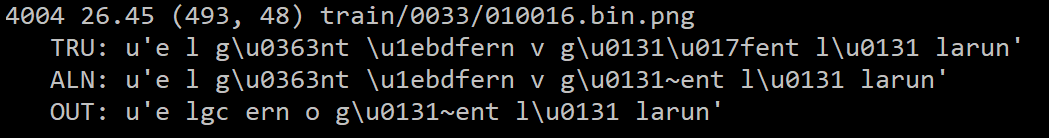
\includegraphics[width=8cm]{screen_output.png}
    \caption{Output d'une itération de l'entraînement}
    \label{API}
\end{figure}

Sur la première ligne se trouve d'abord le numéro de l'itération, puis quelques propriétés de l'image étudiée. L'information se contenant dans le lignes suivantes: \\
- \texttt{TRU} est la solution recherchée \\
- \texttt{ALN} est une version alignée de \texttt{TRU} \\
- \texttt{OUT} est le résultat trouvé par le réseau de neurones \\
Un réseau de neurones idéal aurait les 3 lignes identiques. \\

Afin de lancer la validation d'un modèle et d'avoir le pourcentage d'erreur, on utilise les commandes suivantes : \\
- \texttt{ocropus-rpred -m <ModelName> test/*/*.bin.png} \\
- \texttt{ocropus-errs test/*/*.gt.txt} permet d'évaluer la précision du modèle. \\
- \texttt{ocropus-econf test/*/*.gt.txt} donne les erreurs les plus fréquentes.
On peut ajouter \texttt{-C2} pour une contextualisation des erreurs. \\
\\
Sur ce premier entraînement sans préparations, on obtient une erreur de l'ordre de 27\% au bout de 12 000 itérations ce qui est extrêmement mauvais. En effet, l'ensemble des caractères sortant de l'ordinaire ne sont pas reconnus.


\subsubsection{Entraînement avec les caractères spéciaux}

Afin d'intégrer les caractères spéciaux à la résolution, la méthode est de les ajouter à la liste des caractères, stockée dans \texttt{char.py}. C'est ce que nous avons fait, mais cela n'a rien changé. Nous avons compris par la suite que nos modifications effectuées étaient correctes, mais qu'il faut relancer la commande d'installation pour les prendre en compte ... \\
\texttt{sudo python setup.py install} \\

Ceci nous a permis d'obtenir une première courbe d'erreur satisfaisante. Le tracé est réalisé en analysant les modèles sauvegardés toutes les 1000 itérations, et en inscrivant les résultats dans des documents \texttt{.txt}. Un \textit{parsing} avec python permet de récupérer les informations utiles de ceux-ci. 
Le temps nécessaire pour effectuer 1000 itérations est d'environ 11 minutes sur l'ordinateur que nous avons utilisé pour notre installation \texttt{ocropy}. C'est un portable MSI doté d'une NVIDIA GeForce GTX 1060, le GPU étant le plus important pour entraîner un réseau de neurones.

\begin{figure}[!h] 
	\center
	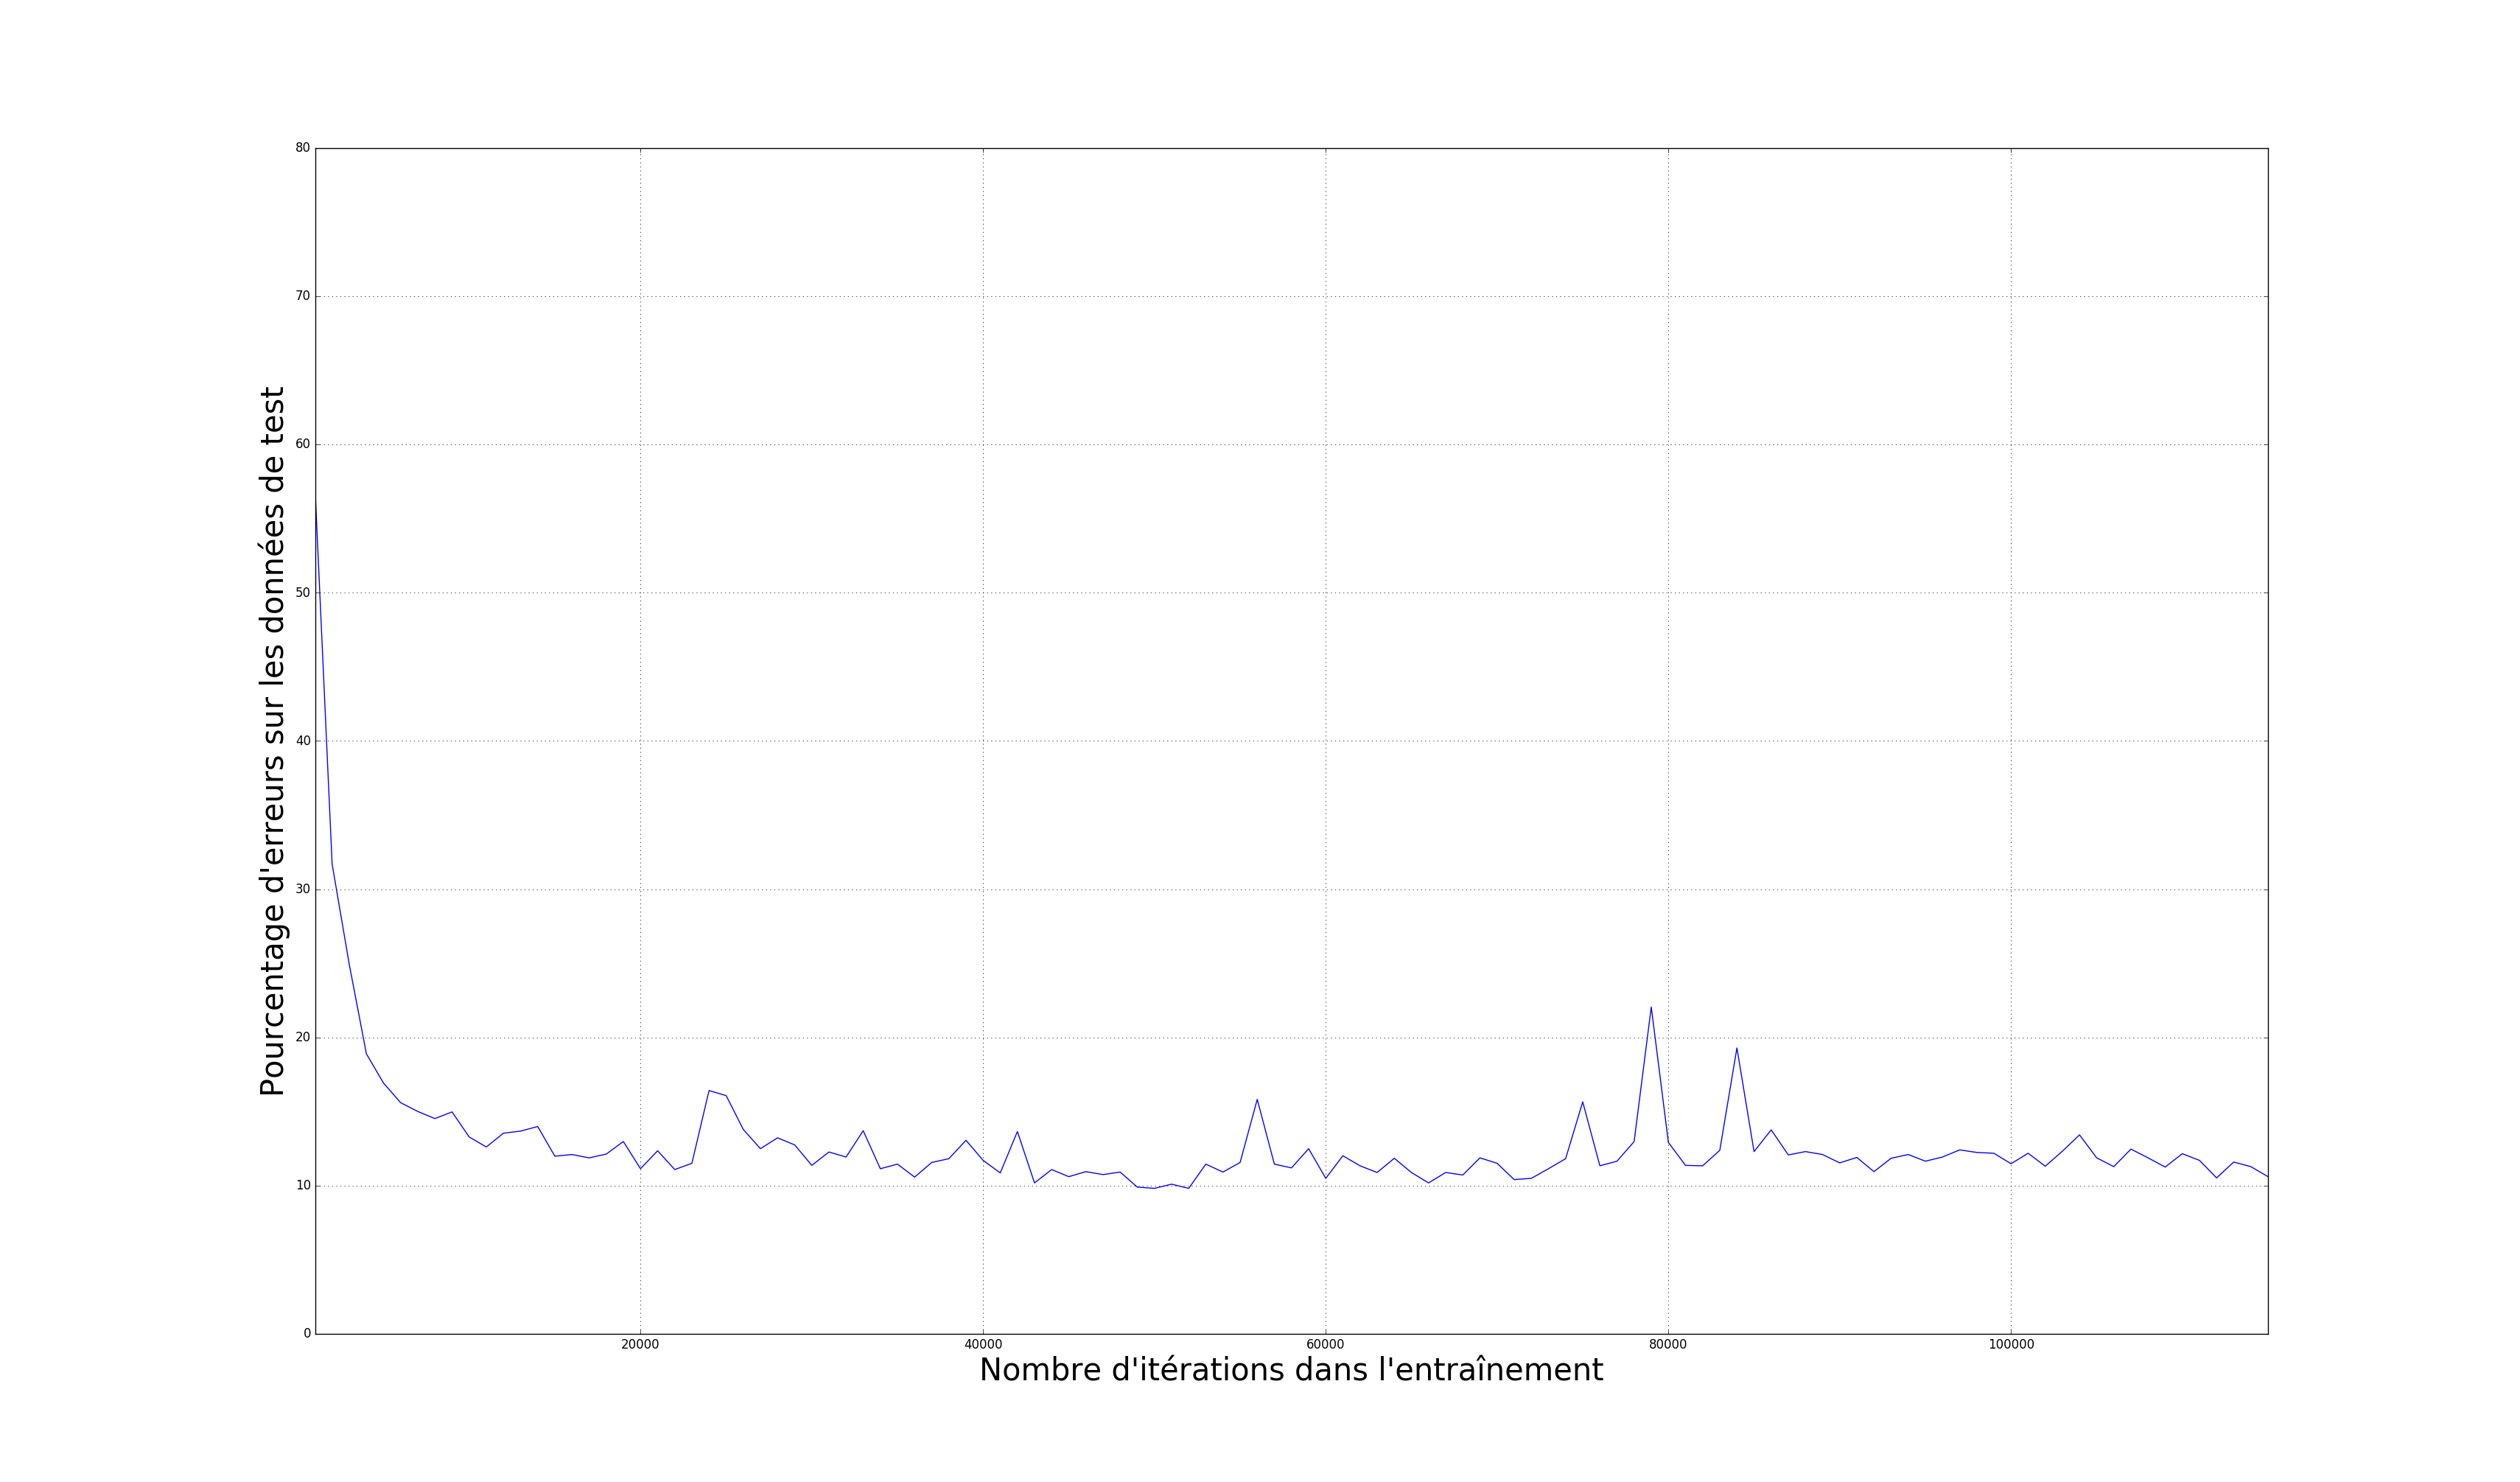
\includegraphics[width=13cm]{error_default.png}
	\caption{Évolution de l'erreur sur les données comportant des caractères spéciaux.}
	\label{err_default}
\end{figure}

Le meilleur modèle est obtenu au bout de $50 000$ itérations, et atteint une erreur de $9.811\%$. Ces résultats sont corrects aux vues de la complexité des données, mais nous pensons pouvoir faire mieux avec un peu de pré-traitement et en modifiant certains paramètres.

\begin{table}[!h]
    \centering
    \begin{tabular}{|l|l|lc|l|l|}
        \hline
        \multicolumn{6}{|c|}{\cellcolor[gray]{0.8}Statistics of the model}                   \\ \hline
        \multicolumn{3}{|l|}{errors}    & \multicolumn{3}{c|}{329}      \\ \hline
        \multicolumn{3}{|l|}{missing}   & \multicolumn{3}{c|}{35}       \\ \hline
        \multicolumn{3}{|l|}{total}     & \multicolumn{3}{c|}{3547}     \\ \hline
        \multicolumn{3}{|l|}{err}       & \multicolumn{3}{c|}{9.275 \%} \\ \hline
        \multicolumn{3}{|l|}{errnomiss} & \multicolumn{3}{c|}{8.289 \%} \\ \hline
    \end{tabular}
    \caption{Output de la commande \texttt{ocropus-errs}}
    \label{t1}
\end{table}

\subsection{Amélioration des modèles}

\subsubsection{Premières normalisation}

Nous avons donc opté pour une nouvelle méthode, consistant à repérer manuellement les caractères utilisés avec les fichiers textes contenant l'information de référence.
On utilise ajoute à la commande d'entraînement la commande suivante : \\
\texttt{-c train/*/*.gt.txt test/*/*.gt.txt} \\
Ceci indiquant qu'on va chercher les symboles dans les \textit{ground truth} disponibles.
Les trois commandes décrites précédemment nous permettent de remarquer qu'au bout de 5000 itérations, l'erreur est descendue à 20\% seulement. La matrice de confusion nous a permis de voir que le caractère \textit{\s} n'était pas reconnu. Ceci étant du à une normalisation de l'unicode effectuée par la l'appel \texttt{-c}. \\
Pour résoudre ce problème nous avons implémenté un script \texttt{Python} remplaçant les caractères de nos données par leur normalisation \textit{NFC}, et ainsi assurer la symétrie entre les données pouvant être apprises et la solution. Cette normalisation est utilisée par \texttt{ocropy} pour traiter les données lors de l'appel de la fonction \texttt{normalize\_text} du module \texttt{common.py}. Cependant, la normalisation du caractère \textit{\s} étant le \textit{s}, déjà présent dans les données, nous l'avons remplacé par un \textit{Z}.

\subsubsection{Analyse des premiers modèles normalisés}

La figure \ref{err_norm} montre les améliorations obtenues grâce à ces premières normalisations.

\begin{figure}[!h] 
    \center
    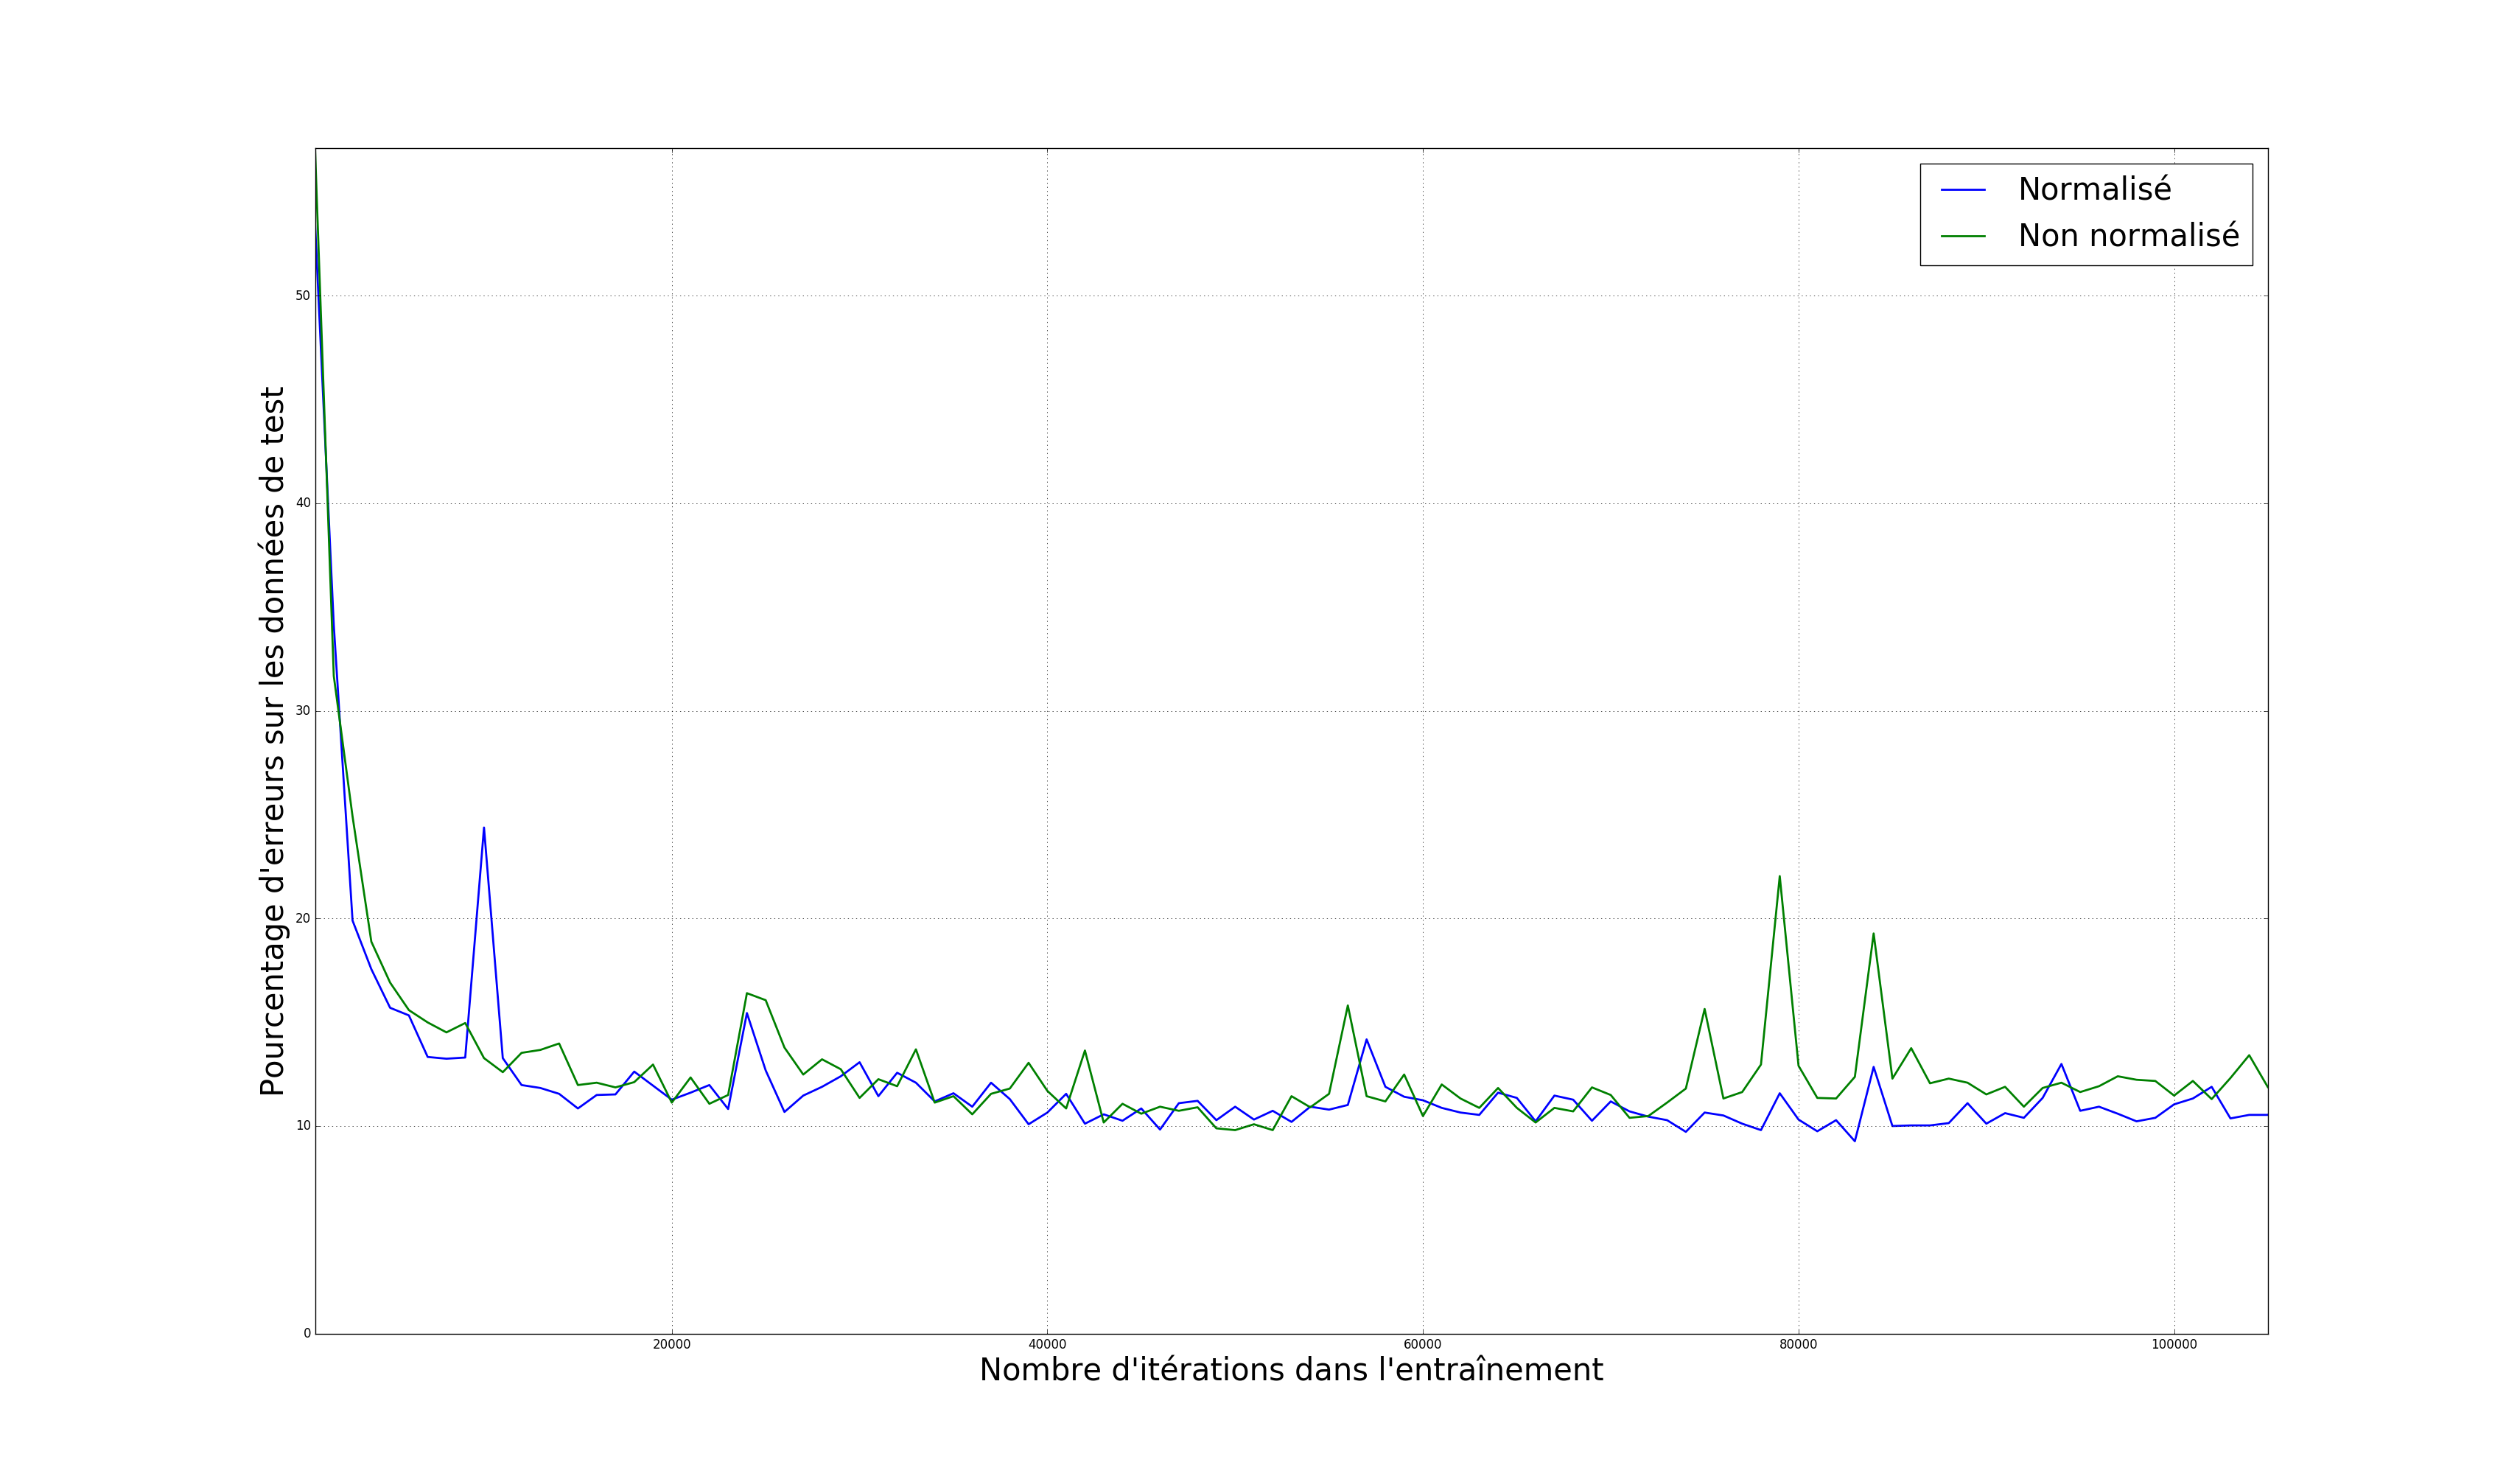
\includegraphics[width=10cm]{error_plot_norm.png}
    \caption{Évolution de l'erreur sur les données normalisées.}
    \label{err_norm}
\end{figure}

La meilleure précision est obtenue pour 83000 itérations, on s'attarde donc un peu plus sur ce modèle particulier pour comprendre les défauts de l'apprentissage. La table \ref{t2} résume les statistiques importantes de ce modèle. \\

\begin{table}[!h]
    \centering
    \begin{tabular}{|l|l|lc|l|l|}
        \hline
        \multicolumn{6}{|c|}{\cellcolor[gray]{0.8}Statistics of the model}                   \\ \hline
        \multicolumn{3}{|l|}{errors}    & \multicolumn{3}{c|}{329}      \\ \hline
        \multicolumn{3}{|l|}{missing}   & \multicolumn{3}{c|}{35}       \\ \hline
        \multicolumn{3}{|l|}{total}     & \multicolumn{3}{c|}{3547}     \\ \hline
        \multicolumn{3}{|l|}{err}       & \multicolumn{3}{c|}{9.275 \%} \\ \hline
        \multicolumn{3}{|l|}{errnomiss} & \multicolumn{3}{c|}{8.289 \%} \\ \hline
    \end{tabular}
    \caption{Résumé de la commande \texttt{ocropus-errs}}
    \label{t2}
\end{table}

Ce qui nous intéresse plus est contenu dans la table \ref{t3} et explique les défauts du réseau de neurones. \\
On distingue 3 types d'erreurs:
\begin{enumerate}[parsep=0.1cm,itemsep=0.1cm,topsep=0.1cm]
    \item Les erreurs sur les espaces;
    \item Les erreurs sur les caractères superscripts;
    \item Les erreurs sur les lettres semblables. 
\end{enumerate}

\noindent Le premier peut sans doute être éliminé avec un peu de traitement des données, le second également mais causerait sans doute de la perte de sens. Le troisième est plus caractéristique de l'écriture puisque les lettres \textit{u, n, m, i et l} se ressemblent souvent.

\begin{table}[!h]
    \centering
    \begin{tabular}{|ccc|ccc|}
        \hline
        \multicolumn{6}{|c|}{\cellcolor[gray]{0.8} Most frequent confusions}                         \\ \hline
        \multicolumn{3}{|c|}{\cellcolor[gray]{0.9}Without context} & \multicolumn{3}{c|}{\cellcolor[gray]{0.9}With context} \\ \hline
        \#       & output       & truth       & \#   & ouput       & truth        \\ \hline
        28       &              &     \_      & 2    & a $\delta$ u  & a\_$\delta$ u        \\
        12       & \_           & \'~         & 2    & uı\_t        & uı\'~ t    \\
        10       & \_           &             & 2    & ıez         &  ıe-       \\
        6        & \_           & \upt{a}      & 1    & e u la lt   & e n la\_lt   \\
        4        & u            & n           & 1    & uı\_ b      & u\'{ı} b        \\
        4        & ı            & \_          & 1    & Ztı         & Ztr         \\
        4        & t            & \_          & 1    & aı\_nZ      & a\'{ı}nZ        \\
        4        & ı            &  r          & 1    & eg ler      & egı\_er      \\
        3        & ı            & u           & 1    & O\_gı       & O gı         \\
        3        & z            & \_          & 1    & e uZ        & e\_uZ        \\ \hline
    \end{tabular}
    \caption{Résumé de la commande \texttt{ocropus-econf}}
    \label{t3}
\end{table}


\subsubsection{Amélioration de la normalisation}

% TODO




\section{Modification des paramètres d'entraînement}

\subsection{Commandes utiles}

Pour modifier l'apprentissage, on peut ajouter une des lignes suivantes à la fin de la commande pour lancer l'entraînement, afin d'en modifier les propriétés. \\
\noindent \texttt{--ntrain <Number>} permet de modifier le nombre d'itérations réalisées dans l'entraînement. Plus ce nombre est grand, meilleur sera le résultat du réseau. Par défaut il vaut $10^6$, mais en général nous nous arrêtons vers $10^5$ itérations.\\
\texttt{--savefreq <Number>} permet de dire le nombre d'itérations entre chaque sauvegarde du modèle. Ceci nous permettra dans la suite de tracer les courbes d'erreur. Le paramètre par défaut est 1000 et est un bon compromis entre la précision des courbes et le temps passé à tester les modèles. \\
\texttt{--lrate <Number>} permet de modifier la vitesse d'apprentissage. \\ (\textit{learning rate}). Un de nos premiers objectifs sera de trouver une bonne valeur de ce paramètre. \\
\texttt{--hiddensize <Number>} permet de modifier un des paramètres de la taille des matrices de notre réseau de neurones. Nous nous intéresserons également à son optimisation. \\

Dans les sous-sections suivantes, nous travaillons avec les données obtenues avec la première normalisation.

\subsection{Modification de la \textit{learning rate}}

On rappelle que la \textit{learning rate}, vitesse d'apprentissage, ou vitesse d'entraînement, est un hyper-paramètre qui caractérise le pas dans la descente du gradient stochastique présente dans le réseau de neurone. Les courbes figure \ref{err_lrate} comparent les modèles pour la valeur par défaut de la vitesse d'apprentissage, $10^{-3}$, et pour une valeur de $10^{-4}$. 

\begin{figure}[!h] 
	\center
	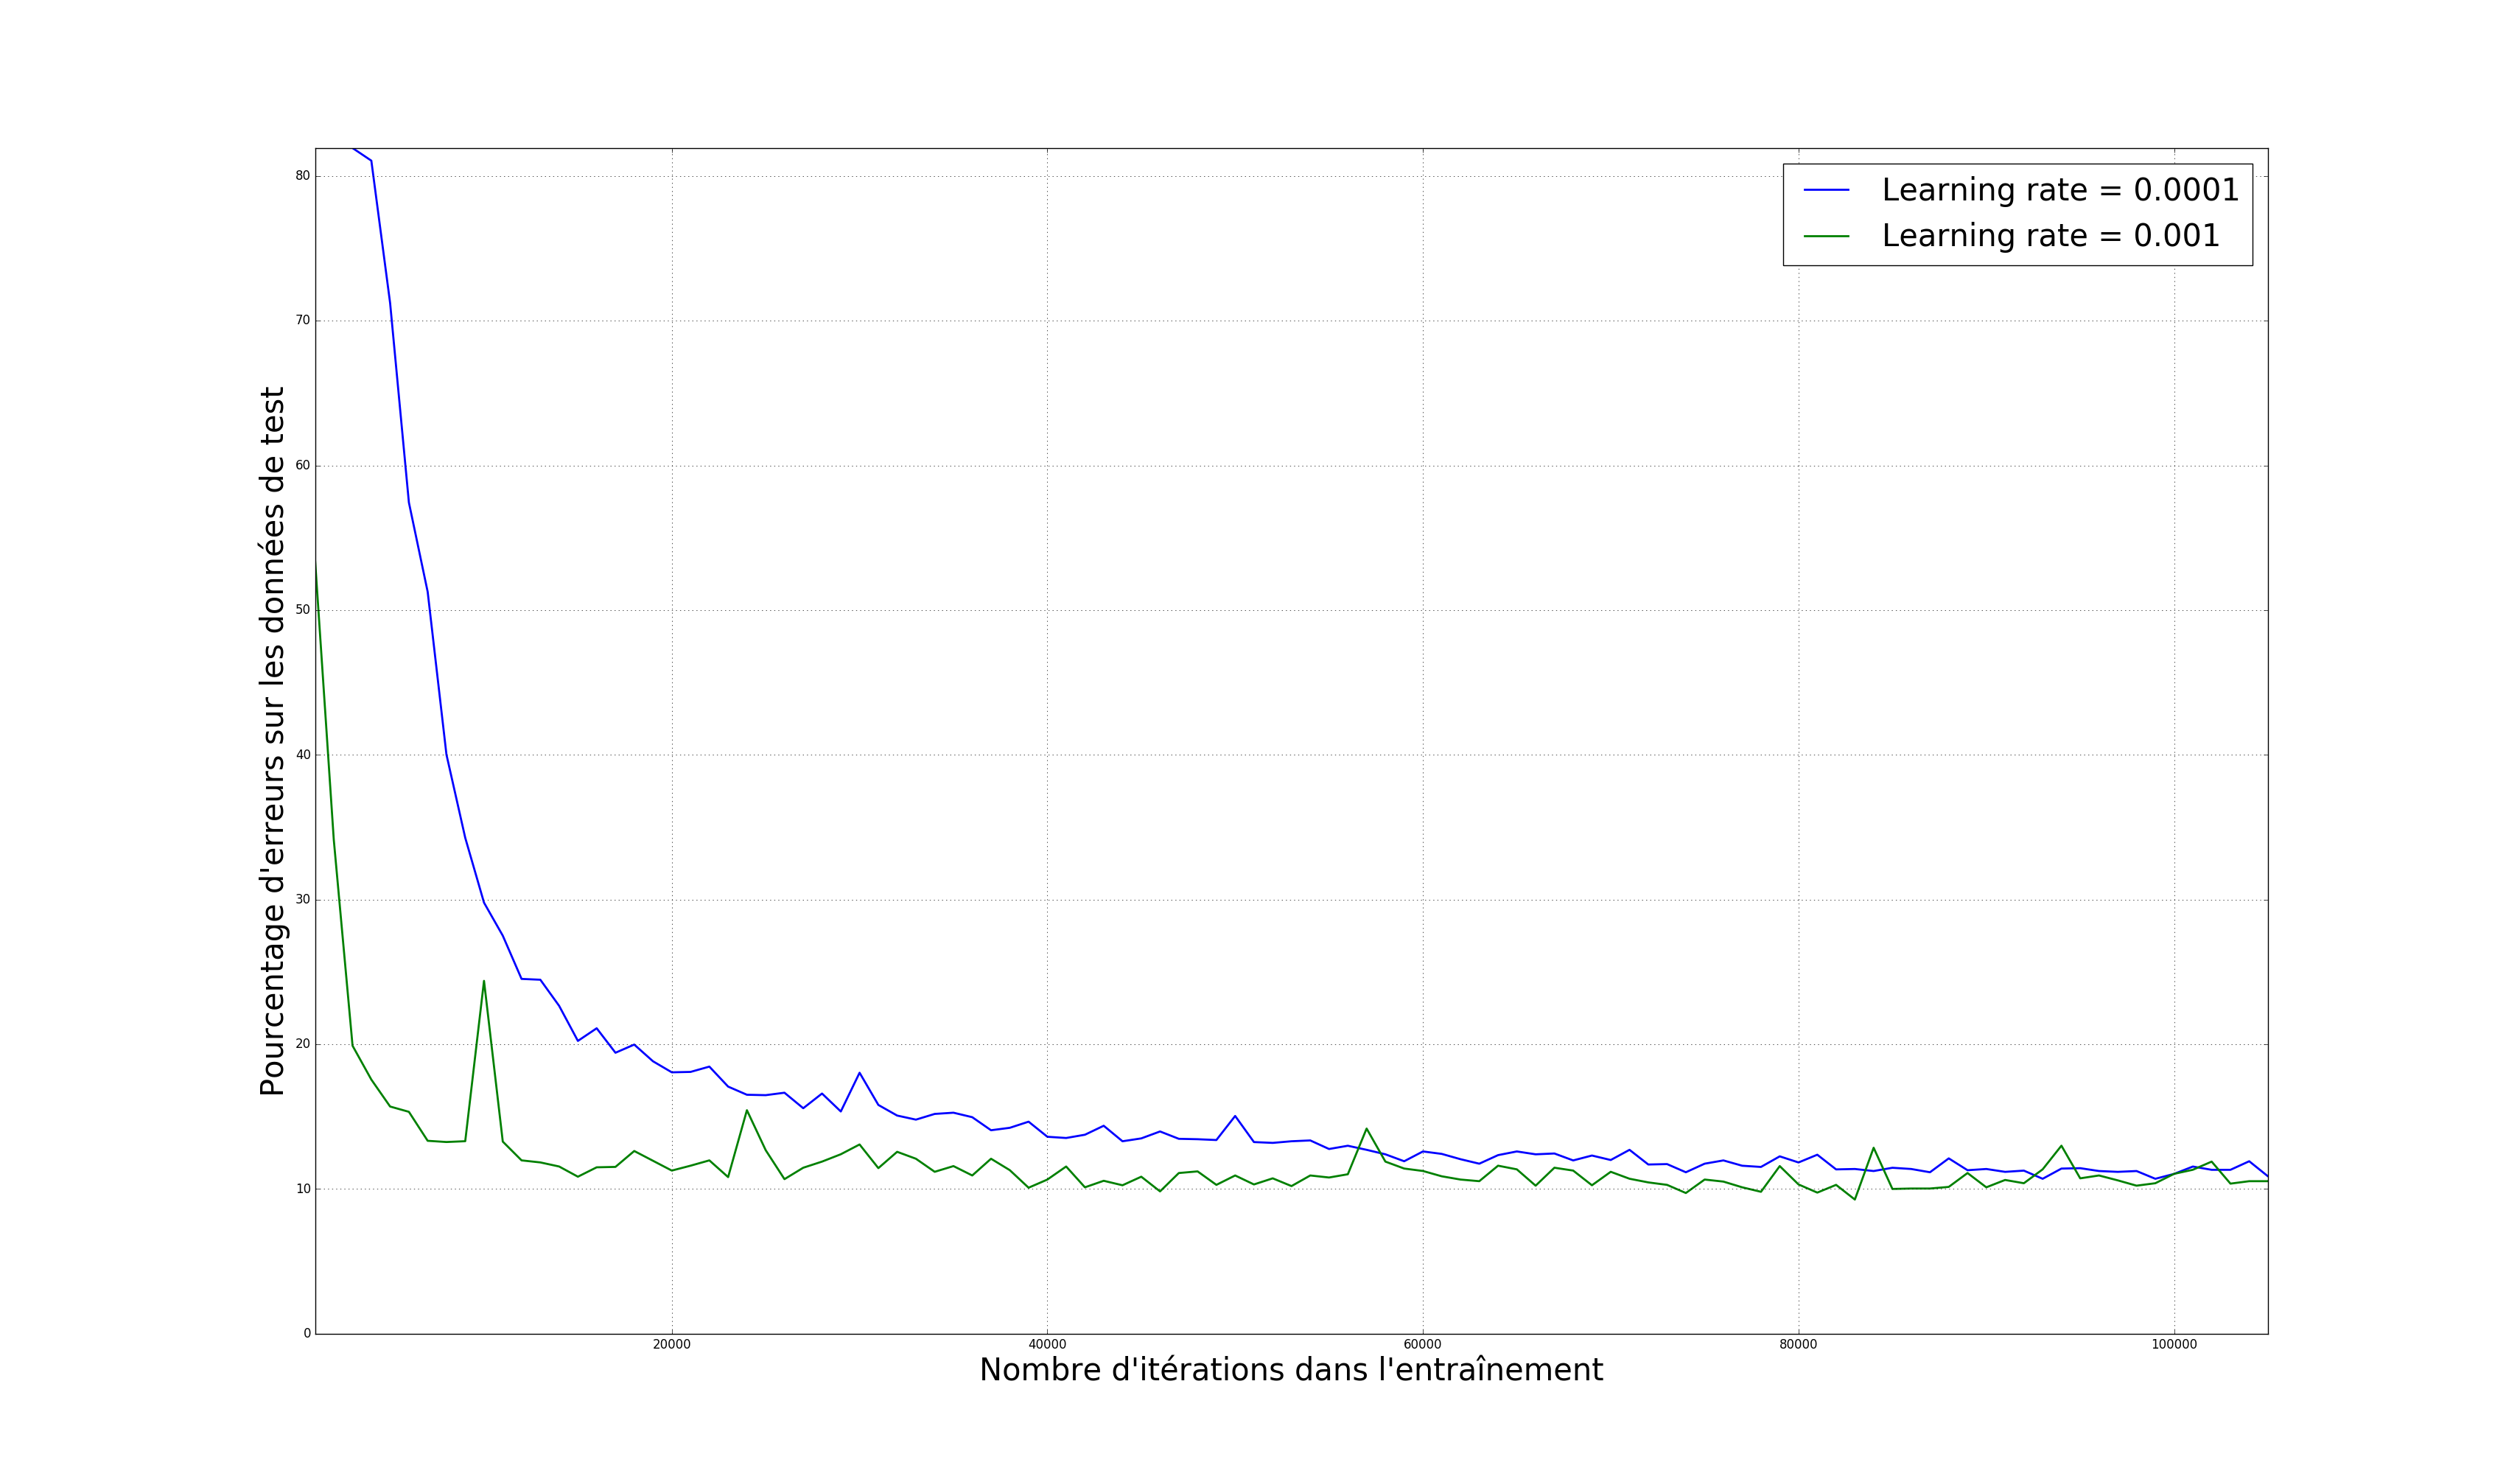
\includegraphics[width=10cm]{error_plot_lrat.png}
	\caption{Évolution de l'erreur pour deux vitesses d'apprentissage différentes.}
	\label{err_lrate}
\end{figure}

On remarque que la courbe au \textit{learning rate} plus faible est plus lente à converger, mais plus régulière. En raison de cette stabilité, le meilleur modèle, obtenu pour 133000 itérations a un taux d'erreur de 9.949\% pour la \textit{learning rate} la plus faible, contre 9.275\% au bout de 83000 itérations dans l'autre cas. C'est pourquoi nous garderons une \textit{learning rate} de $10^{-3}$ dans la suite.

\subsection{Modification de la taille du réseau}

Le paramètre sur lequel on joue ici est le paramètre définissant le nombre de \textit{hidden state}. Ce sont les variables que le \textit{LSTM} utilise pour garder une trace du temps. C'est la partie récurrente du réseau. L'influence de ce paramètre est présentée figure \ref{err_size}.

\begin{figure}[!h] 
	\center
	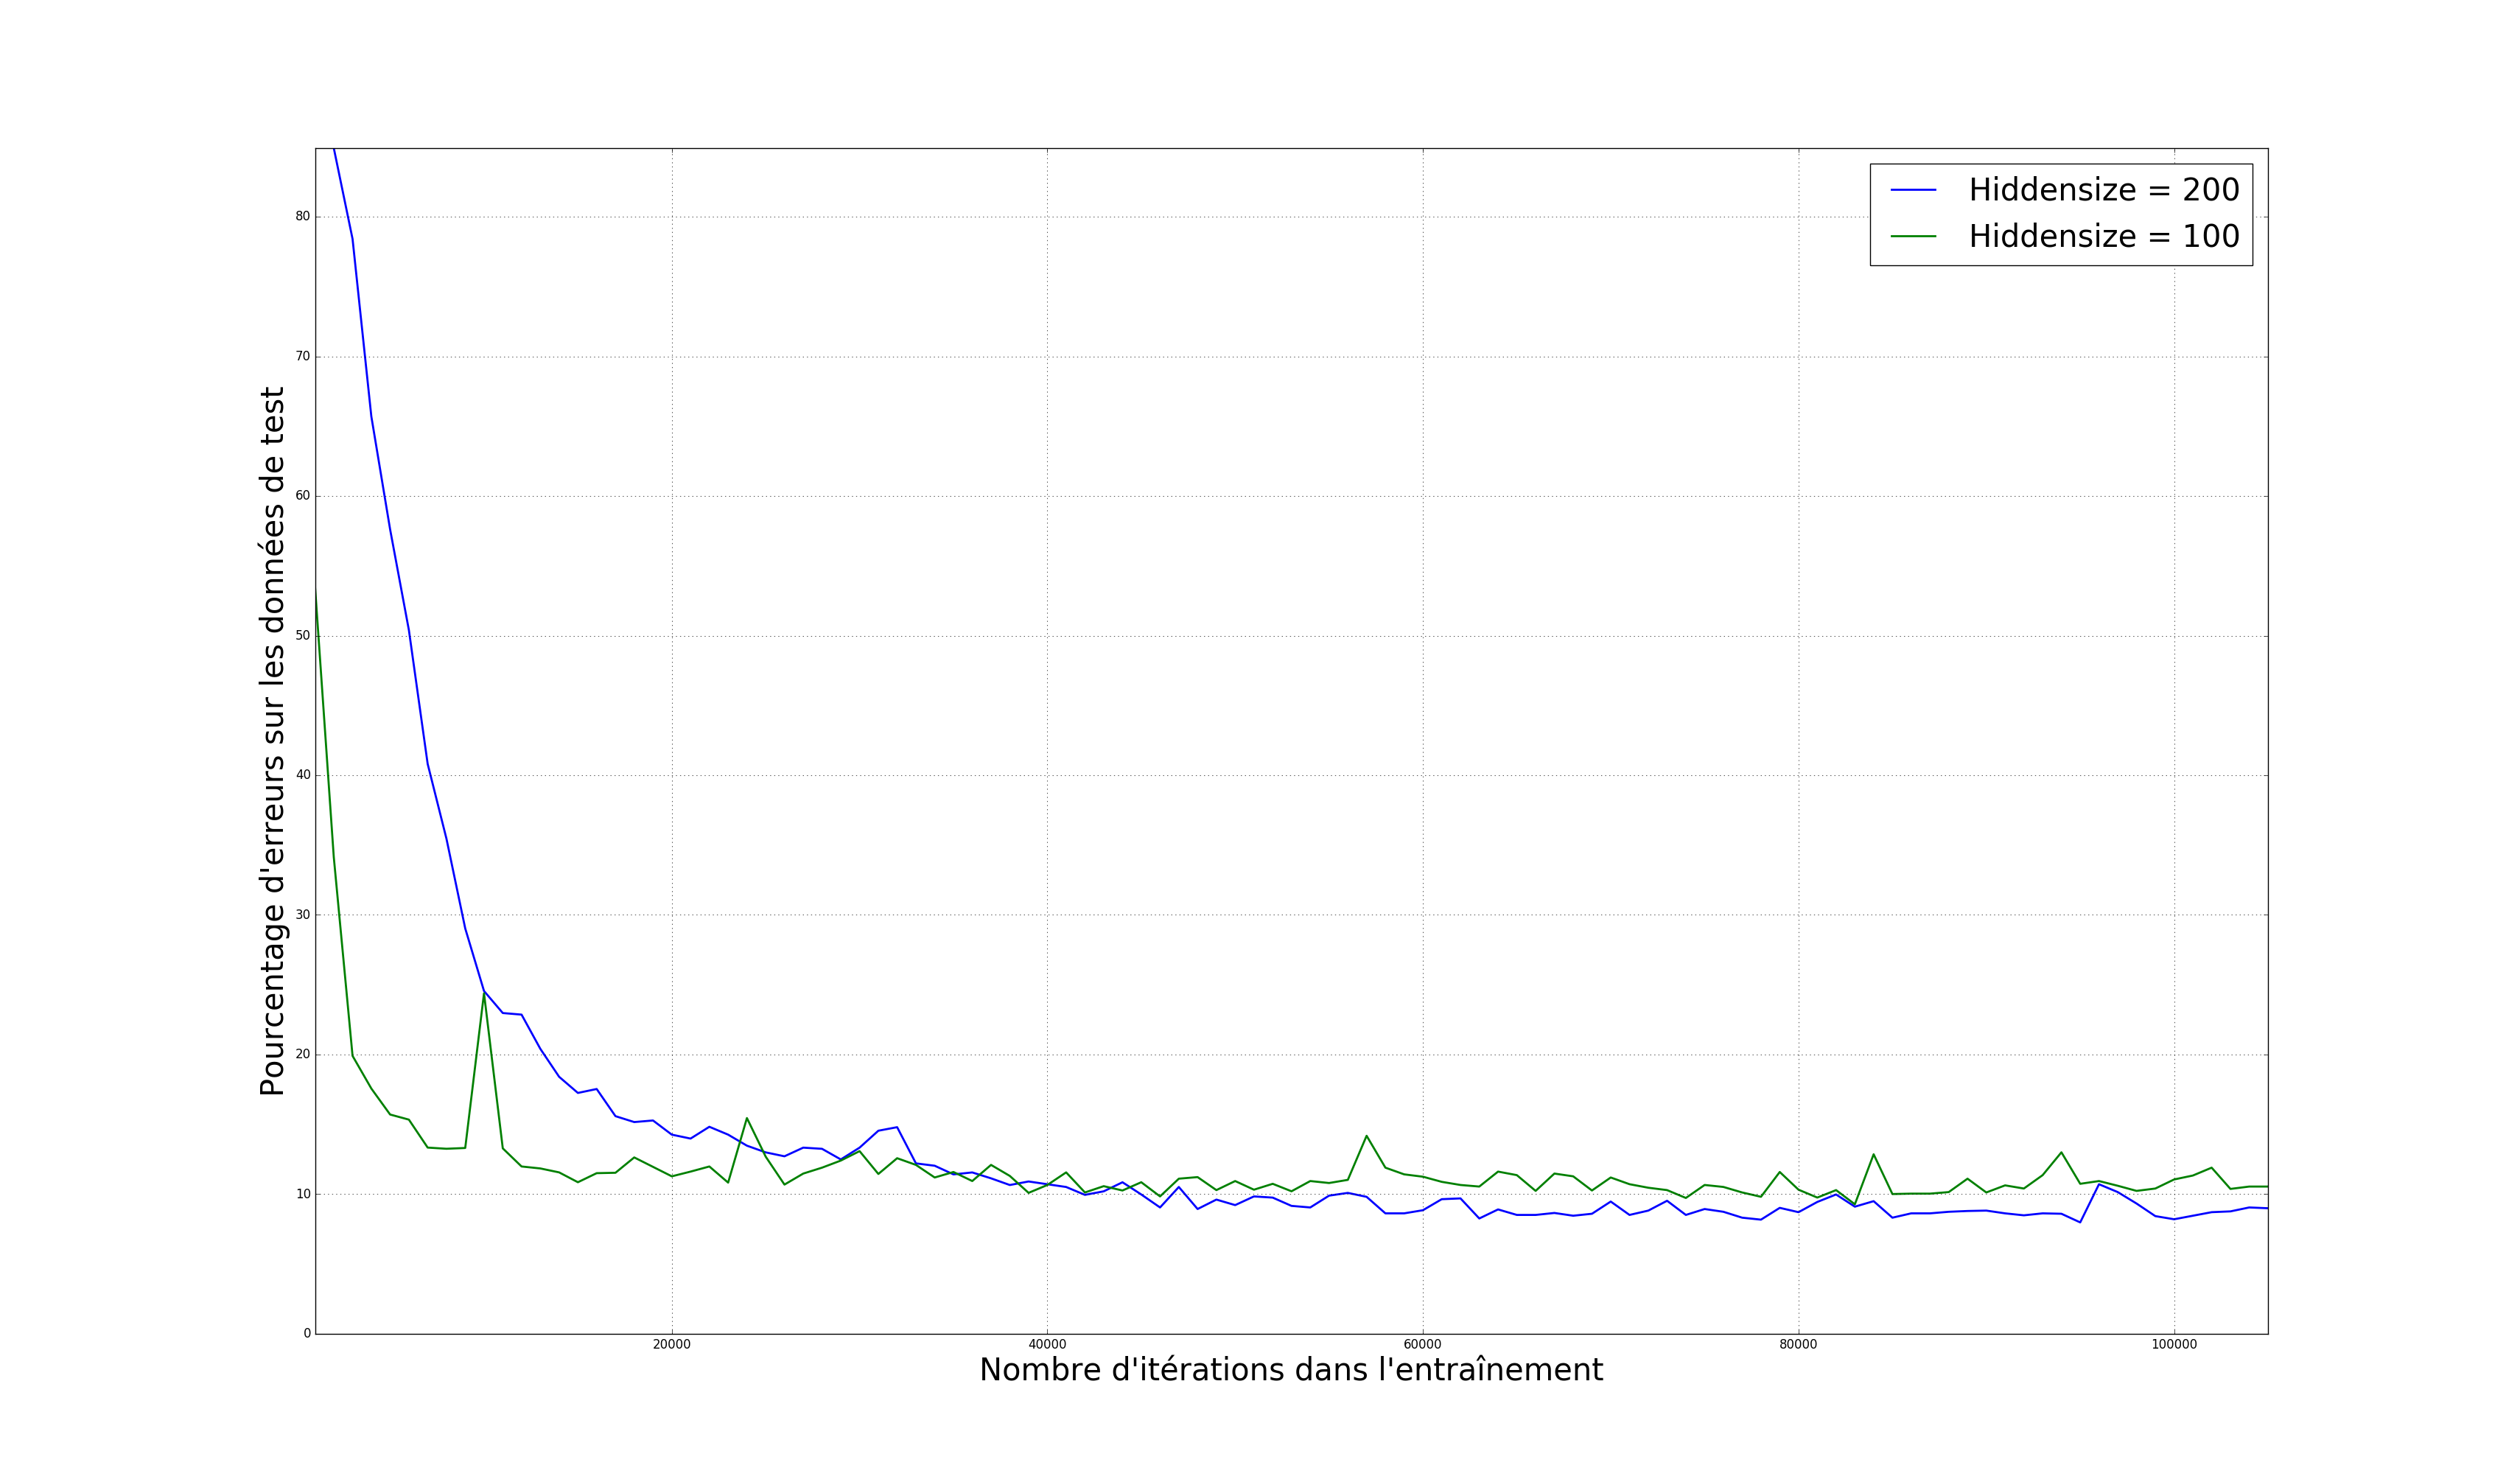
\includegraphics[width=10cm]{error_plot_size.png}
	\caption{Évolution de l'erreur pour deux tailles de réseau différentes.}
	\label{err_size}
\end{figure}

On remarque que les résultats sont meilleurs quand on augmente ce paramètre. La convergence est un peu plus lente en nombre d'itérations, cependant, nous sommes passé de 12 à 18 minutes de temps de calcul nécessaire pour effectuer 1000 itérations. Le meilleur modèle que nous avons obtenu a une erreur de 7.976\%, atteinte pour 95000 itérations, soit plus d'un jour d'entraînement. 
\section{Commandes bash utilisées}

\begin{lstlisting}[language=bash]
    ocropus-rpred -m test3-00005000.pyrnn test/*/*.bin.png
    ocropus-errs test/*/*.gt.txt
\end{lstlisting}

\begin{lstlisting}[language=bash]
    ocropus-rtrain -o <modelname> <training-dir>/*/*.bin
    ocropus-rtrain -o myModel -d 1 train/*/*.bin.png
\end{lstlisting}

\begin{lstlisting}[language=bash]
    for i in test8/*.pyrnn.gz; do
        echo "\$i" >> results.txt
        ocropus-rpred -m \$i test/*/*.bin.png
        ocropus-errs test/*/*.gt.txt >> results.txt
        echo "\$i" >> index.txt
    done
\end{lstlisting}

\begin{lstlisting}[language=bash]
    sudo python setup.py install
\end{lstlisting}

\begin{lstlisting}[language=bash]
    ocropus-rtrain -o test8 train2/*/*.bin.png --load test8-00086000.pyrnn
\end{lstlisting}

\begin{lstlisting}[language=bash]
    ocropus-rtrain -c train/*/*.gt.txt test/*/*.gt.txt -o test7 train/*/*.bin.png --load test7-00073000.pyrnn
\end{lstlisting}

\begin{lstlisting}[language=bash]
    ocropus-rpred -m test8-00050000.pyrnn test/*/*.bin.png
\end{lstlisting}

\end{document}

\subsection{Modification de la vitesse d'apprentissage}

\subsection{Modification de la taille du réseau}

\end{document}